\renewcommand{\assert}[1]{\hoareassert{#1}}
\renewcommand{\kw}[1]{\textbf{#1}}

\section{Algorithmen: Hoare-Kalkül}

\subsection{Algorithmen}
\begin{frame}{Algorithmen}
	\begin{block}{Definition}
		Ein Algorithmus ist...
		\begin{itemize}[<+->]
			\item Eine endliche Beschreibung
			\item aus elementaren Anweisungen, 
			\item die deterministisch ($=$ ohne Zufall!) ausgeführt werden.\\
				{\small (Manchmal auch gemischt mit (Pseudo-)Zufallselementen)}
			\item Eine endliche Eingabe gibt endliche Ausgabe...
			\item in endlich vielen Schritten.
			\item Das funktioniert für beliebig große Eingaben und
			\item ist nachvollziehbar bzw. verständlich.
		\end{itemize}
	\end{block}
	\pause[8]
	Woher wissen wir, ob ein Algorithmus korrekt ist?
\end{frame}

\begin{frame}{Korrektheit}
	Einige Algorithmen haben besonders hohe Anforderungen an ihre Korrektheit:
	Banking-Server, Airbag-Steuerprogramm, Herzschrittmacher, ...
	\bigskip

	
	Korrektheit garantieren?\pause
	\begin{itemize}
		\item Testen? \pause Was, wenn wir einen Sonderfall vergessen? \pause
		\item Alle Eingaben testen? \pause Oft nicht möglich. \pause
		\item Formal beweisen: \textbf{Hoare-Kalkül} \pause
	\end{itemize}
	
	\begin{block}{In der Praxis}
		Theoretisch müsste die komplette Werkzeugkette bewiesen werden:
		Programm, Compiler, Prozessor...\\
		Oft wird bei Compilern nur “Proven in use” benutzt: Compiler, bei
		denen seit Jahren keine Fehler gefunden wurden.
	\end{block}
	
\end{frame}

\subsection{Hoare-Kalkül}
\begin{frame}{Der Hoare-Kalkül}
	\begin{block}{Definition}
		Ein \emph{Hoare-Tripel} ist ein Tripel $\set{P}\ S \ \set{Q}$ mit einem Programmstück $S$ und prädikatenlogischen \emph{Zusicherungen} $P,Q$.
	\end{block}
	\pause
	$P = $ Vorbedingung vor der Ausführung \\
	$Q = $ Nachbedingung nach der Ausführung\\
	$S = $ Programmstück
	
	\pause
	\bigskip
	Dabei: Wir betrachten nur \enquote{relevante} Interpretationen:
	\begin{itemize}[<+->]
		\item Fester Grundbereich (explizit angegeben oder implizit ableitbar)
		\item Funktionen und Relationen \enquote{wie üblich} interpretiert.
		\item Konstanten beliebig, als \enquote{Eingabe} des Programms.\\
		Muss also für alle Möglichkeiten (also Eingaben) gelten.
	\end{itemize}
\end{frame}

%TODO
\begin{frame}{Der Hoare-Kalkül}
	\begin{block}{Definition}
		Ein Hoare-Tripel $\htr{P}{S}{Q}$ ist \textbf{gültig}, wenn für jede relevante Interpretation $I$ und jede Variablenbelegung $\beta$ gilt:\\
		Wenn vor der Ausführung $\val_{D,I,\beta}(P)=\W$ ist und die Ausführung von $S$ für $I$ und $\beta$ mit der neuen Variablenbelegung $\beta'$ endet, dann gilt anschließend auch $\val_{D,I,\beta'}(Q)=\W$. \\
		\medskip
		Auf Deutsch: \\
		$\htr{P}{S}{Q}$ ist \textbf{gültig} \Gdw Wenn anfangs $P$ gilt, wir $S$ ausführen und dann zum Schluss $Q$ gilt.
	\end{block}
\end{frame}

\begin{frame}{Hoare-Tripel}
	\begin{Beispiel}
        \vspace{0.2\baselineskip}
		\begin{columns}[T] 
			\begin{column}[T]{.4\textwidth} 
				$\assert{x = 5}$ \\
				$x \gets x + 1$ \\
				$\assert{x = 6}$ \\
				ist gültig.  \\
				
				\bigskip
				$\assert{x = 5}$ \\
				$x \gets x + 1$ \\
				$\assert{x = 42}$ \\
				ist nicht gültig.
			\end{column}
			\begin{column}[T]{.4\textwidth} 
				\pause
				$\assert{z = 5}$ \\
				$x \gets x + 1$ \\
				$\assert{z = 5}$ \\
				ist gültig.  \\
				
				
				\bigskip
				$\assert{x = x}$ \\
				$\kw{while } 1 = 1 \kw{ do } x \gets x + 1 \kw{ od}$ \\
				$\assert{\W = \F}$ \\
				ist gültig (Q wird nie erreicht).
			\end{column}
		\end{columns}
	\end{Beispiel}
	\medskip
	\pause
	\begin{block}{Hoare-Kalkül}
		Der \emph{Hoare-Kalkül} definiert Regeln, wie gültige \emph{Hoare-Tripel} schrittweise aus Axiomen abgeleitet werden können.
	\end{block}
\end{frame}


\begin{frame}{HT-A}
	\begin{block} {Axiom HT-A \quad „Assignment“}
		$$ \{\sigma_{\{\text{x/E}\}} (Q)\} \quad x \leftarrow E \quad \{Q\} $$
	\end{block}
	\pause
	Nach einer Zuweisung gilt jede Aussage für die Variable, welche vorher für die rechte Seite der Zuweisung galt.
	\begin{itemize}
		\item $\sigma_{\{\text{x/E}\}} (Q) $ ist die Aussage, die dadurch entsteht, dass man in Q jedes freie Vorkommen von x durch E ersetzt.
		\item \textbf{Achtung}: $\sigma_{\{\text{x/E}\}}$ muss kollisionfrei sein!
	\end{itemize}
	
	\begin{Beispiel}
		$\{ x + 1 = 43\} \ y \gets x + 1\ \{y = 43 \}$ ist gültig. \pause (Bzw. umgeformt \\
		$\{ x = 42 \} \ y \gets x + 1\ \{y = 43 \}$).
	\end{Beispiel}
	
\end{frame}

\begin{frame}{HT-E}
	\begin{block}{Regel HT-E}
		Wenn $\{P\}\ S\ \{Q\}$ gültig ist, dann auch $\{P'\}\ S\ \{Q'\}$ mit $P' \impl P$ und $Q \impl  Q'$.
	\end{block}
	\pause
	Heißt: Vorbedingungen können stärker, Nachbedingungen können schwächer werden.

	\begin{Beispiel}
		Aus $\{ x = 41\} \ x \gets x + 1\ \{x = 42 \}$ können wir \\
		$\{ x + y = 42 \land y = 1 \} \ x \gets x + 1\ \{x \in \R \}$ ableiten.
	\end{Beispiel}
\end{frame}

\begin{frame}{HT-S}
	\begin{block}{Regel HT-S \quad „Sequence“}
		Wenn $\{P\}\ S_1\ \{Q\}$ und $\{Q\}\ S_2\ \{R\}$ gültig sind, dann auch $\{P\}\ S_1;  S_2\ \{R\}$. 
	\end{block}
	\pause
	\impl Hoare-Tripel können transitiv zusammengefasst werden.
\end{frame}

\begin{frame}
	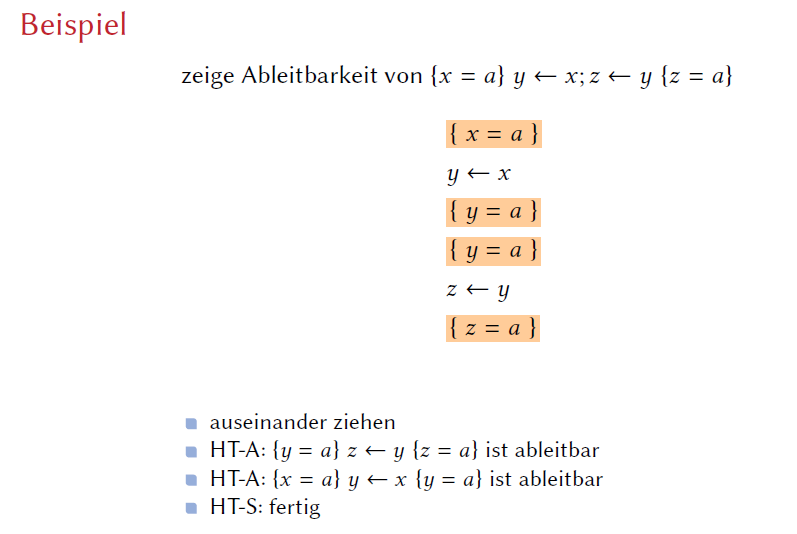
\includegraphics[scale=0.5]{hoare/bsp1}
\end{frame}

\begin{frame}{HT-I}
	\begin{minipage}{0.4\linewidth}
		\begin{align*}
			&\assert{ P } \\
			& \textbf{if } B \textbf{ then} \\
			&\hspace{2em} \assert{ P \wedge B } \\
			&\hspace{2em} S_1 \\
			&\hspace{2em} \assert{ Q }\\
			&\textbf{else} \\
			&\hspace{2em} \assert{ P \wedge \neg B } \\
			&\hspace{2em} S_2 \\
			&\hspace{2em} \assert{ Q }  \\
			&\textbf{fi}\\
			&\assert{Q }
		\end{align*}
	\end{minipage}
	\begin{minipage}{0.55\linewidth}
		\begin{block}{Regel HT-I \quad „If“}
			$\textbf{if } B\text{ } \textbf{ then } S_1 \textbf{ else } S_2 \textbf{ fi}$
			\smallskip
			\begin{itemize}
				\item Wenn $\{ P \wedge B \}\ S_1\ \{ Q \}$ gültig 
				\item und $\{ P \wedge \neg B \}\ S_2\ \{ Q \}$ gültig
				\item dann auch \\ $\{ P \} \textbf{ if } B \textbf{ then } S_1 \textbf{ else } S_2 \textbf{ fi } \{ Q \} $ gültig
			\end{itemize}
		\end{block}
%		\emph{HT4 : } $\textbf{if } B\text{ } \textbf{then } S_1 \textbf{ else } S_2 \textbf{ fi}$
%		\begin{itemize}
%			\item Wenn $\{ P \wedge B \} S_1 \{ Q \}$ gültig 
%			\item Wenn $\{ P \wedge \neg B \} S_2 \{ Q \}$ gültig
%			\item dann auch $\{ P \} \textbf{ if } B \textbf{ then } S_1 \textbf{ else } S_2 \textbf{ fi} \{ Q \} $ gültig
%		\end{itemize}
	\end{minipage}
\end{frame}

\begin{frame}{Beispiel: Berechnung von $\vert x \vert$}
	
	
	\begin{minipage}{0.5\linewidth}
		Erinnerung:
		\vspace{-1\baselineskip}
		\begin{align*}
		&\assert{ P } \\
		& \textbf{if } B \textbf{ then} \\
		&\hspace{2em} \assert{ P \wedge B } \\
		&\hspace{2em} S_1 \\
		&\hspace{2em} \assert{ Q }\\
		&\textbf{else} \\
		&\hspace{2em} \assert{ P \wedge \neg B } \\
		&\hspace{2em} S_2 \\
		&\hspace{2em} \assert{ Q }  \\
		&\textbf{fi}\\
		&\assert{Q }
		\end{align*}
	\end{minipage}
	\begin{minipage}{0.4\linewidth}
		\begin{align*}
		&\assert{ x \in\R} \\
		&\textbf{if } x < 0 \textbf{ then } \\
		&\hspace{2em} \assert{ \visible<6->{ x\in\R\wedge x < 0 } } \\
		&\hspace{2em} \assert{ \visible<5->{ {-x} = \vert x \vert } } \\
		&\hspace{2em}  z \gets -x   \\
		&\hspace{2em} \assert{ \visible<2->{ z = \vert x \vert } } \\
		&\textbf{else} \\
		&\hspace{2em} \assert{ \visible<4->{ x\in\R\wedge x\geq 0 } } \\
		&\hspace{2em} \assert{ \visible<3->{ x = \vert x \vert } } \\
		&\hspace{2em} z \gets x \\
		&\hspace{2em} \assert{ \visible<2->{ z = \vert x \vert } } \\
		&\textbf{fi} \\
		&\assert{ z = \vert x \vert } 
		\end{align*}
	\end{minipage}
\end{frame}

\begin{frame}{Aufgabe}
	\vspace{-10mm}
	  \begin{align*}
	&\assert{x=a \land y=b}  \\
	&\kw{if } x>y \kw{ then } \\
	&\hspace{2em} \assert{ \dots\ } \\
	&\hspace{2em}  z \gets y  \\
	&\hspace{2em} \assert{ \dots\ } \\
	&\kw{else } \\
	&\hspace{2em} \assert{ \dots\ } \\
	&\hspace{2em}  z \gets x  \\
	&\hspace{2em} \assert{ \dots\ } \\
	&\kw{fi } \\
	&\assert{z=\min(a,b)}
	\end{align*}
\end{frame}

\begin{frame}{Lösung}	
	\vspace{-2.5\baselineskip}
	\begin{alignat*}{2}
	&\assert{x=a \land y=b}  \\
	&\kw{if } x>y \kw{ then } \\
	&\hspace{2em} \assert{x=a \land y=b \land x>y} \\
	&\hspace{2em} \assert{y=\min(a,b)} \\
	&\hspace{2em}  z \gets y  \\
	&\hspace{2em} \assert{z=\min(a,b)} \\
	&\kw{else } \\
	&\hspace{2em} \assert{x=a \land y=b \land  \lnot (x>y)} \\
	&\hspace{2em} \assert{x=\min(a,b)} \\
	&\hspace{2em}  z \gets x  \\
	&\hspace{2em} \assert{z=\min(a,b)} \\
	&\kw{fi } \\
	&\assert{z=\min(a,b)}
	\end{alignat*}
\end{frame}


\mycomment{
%TODO: Lösung!!!
\begin{frame}{Jetzt seid ihr dran}
	\begin{align*}
	& z \gets x + y \\
	& z \gets z / 2 \\
	&\textbf{if } x \mod 2 = 0 \textbf{ then } \\
	&\hspace{2em} y \gets x + x \\
	&\hspace{2em} y \gets y / 4 \\
	&\textbf{else} \\
	&\hspace{2em} y \gets x - 1 \\
	&\hspace{2em} y \gets y / 2 \\
	&\textbf{fi} \\
	& z \gets z \· y \\
	&\assert{ z = div_2(a) \· (a+b)/2 } % WTF is div_2 ? => (2 `div`) ? a, b vs. x, y?
	\end{align*}
\end{frame}	
}


%\begin{frame}
%	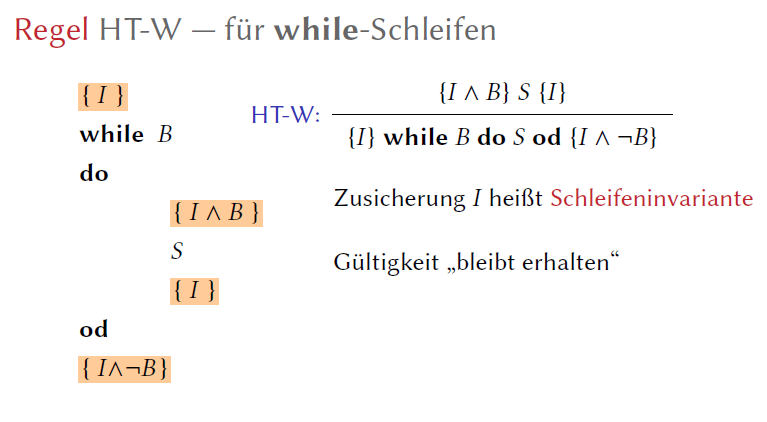
\includegraphics[scale=0.5]{hoare/htw}
%\end{frame}

\subsection{HT-W, Schleifeninvarianten}
\begin{frame}{HT-W}
	\begin{columns}[T] 
		\begin{column}[T]{.4\textwidth} 
			\vspace{-2\baselineskip}
			\begin{align*}
			&\assert{I} \q3uad \text{„Schleifeninvariante“} \\
			&\kw{while } B \kw{ do } \\
			&\qquad \assert{I \land B} \\
			&\qquad S \\
			&\qquad \assert{I} \\
			&\kw{od} \\
			&\assert{I \land \lnot B}
			\end{align*}
			\vspace{-1\baselineskip}
		\end{column}
		\begin{column}[T]{.4\textwidth} 
			\begin{block}{Regel HT-W \quad „While“}
				Wenn \htr{$I \land B$}{$S$}{$I$} gültig ist, dann ist auch die ganze \kw{while}-Schleife (s. links) gültig
			\end{block}
		\end{column}
	\end{columns}
	
	\pause
	\begin{block}{Schleifeninvarianten}
		\begin{itemize}
			\item sind Aussagen, die zu Beginn und Ende jedes Schleifendurchganges gültig sind
			% \item helfen, die Korrektheit eines Programmes zu beweisen
			\item muss man ebenfalls beweisen 
			\item garantieren nicht die Korrektheit des Programms:\pause \\
			 Terminierung der Schleife muss zusätzlich gezeigt werden! (nicht in GBI)
		\end{itemize}
	\end{block}
\end{frame}
	
\begin{frame}{Beispiel Schleifeninvarianten}
	\begin{columns}
    	\begin{column}[T]{0.49\linewidth}
        	\begin{align*}
        		&\assert{x=a \land y=b}  \\
        		&\assert{ \dots\ } \\
        		&\kw{while } y\not=0 \kw{ do } \\
        		&\qquad\assert{ \dots } \\
        		&\qquad y \gets y-1 \\
        		&\qquad\assert{ \dots } \\
        		&\qquad x \gets x+1 \\
        		&\qquad\assert{ \dots\ } \\
        		&\kw{od } \\
        		&\assert{ \dots\ } \\ 
        		&\assert{x=a+b} \\
        	\end{align*}
    	\end{column} 

        \pause
        
    	\begin{column}[T]{0.5\linewidth}
    			\bigskip
    			\begin{block}{Wertetabelle für $a=3$ und $b=4$}
    				\centering
    				\medskip
    				\begin{tabular}{c|cc}	 
    					Durchlauf $i$ & $x$ & $y$ \\ 
    					\hline 
    					0 & 3 & 4 \\
    					1 & 4 & 3 \\
    					2 & 5 & 2 \\
    					3 & 6 & 1 \\
    					4 & 7 & 0 \\
    				\end{tabular}
    			\end{block}
    			\pause
    			Schleifeninvariante: $$ x + y = a + b $$ 
    	\end{column}
	\end{columns}
\end{frame}

\begin{frame}{Beispiel Schleifeninvarianten – Lösung}
	\begin{minipage}{.4\linewidth}
		Erinnerung HT-W:
		\vspace{-.4\baselineskip}
		\begin{align*}
		&\assert{I}  \\
		&\kw{while } B \kw{ do } \\
		&\qquad \assert{I \land B} \\
		&\qquad S \\
		&\qquad \assert{I} \\
		&\kw{od} \\
		&\assert{I \land \lnot B}
		\end{align*}
	\end{minipage}
	\begin{minipage}{.4\linewidth}
		\begin{align*}
		&\assert{x=a \land y=b }  \\
		&\assert{ x+y=a+b }  \\
		&\kw{while } y\not=0 \kw{ do } \\
		&\qquad\assert{x+y=a+b \land y\not=0 }  \\
		&\qquad\assert{x+1+y-1=a+b } \\
		&\qquad y \gets y-1 \\
		&\qquad\assert{x+1+y = a+b} \\
		&\qquad x \gets x+1 \\
		&\qquad\assert{ x+y = a+b} \\
		&\kw{od } \\
		&\assert{ x+y = a+b \land y=0 } \\
		&\assert{x=a+b} \\
		\end{align*}
	\end{minipage}
	
\end{frame}

\begin{frame}{Exkurs: Schl.-Inv. mit Vollst. Induktion}
	Wir zeigen mit vollständiger Induktion die Gültigkeit der Schleifeninvariante. Dabei sei $i$ die Anzahl der bisher durchgelaufenen Schleifendurchläufe.\\
	
	\emph{Behauptung}: $$ \forall\ i \in \{0,...,b\} : x_i + y_i = a+b $$ \pause
	\begin{block}{Induktionsanfang}
		Für $i=0$ gilt $ x_0+y_0 = a+b $ nach Vorbedingung.
	\end{block} \pause 
	\begin{block}{Induktionsvorrausetzung}
		Für ein beliebig aber festes $i\in \{0,...,b\}$ gelte die Behauptung.
	\end{block}
\end{frame}

\begin{frame}{Exkurs: Schl.-Inv. mit Vollst. Induktion}
	\vspace{-2\baselineskip}
	\begin{align*}
	&\assert{x=a \land y=b}  \\
	&\assert{ x+y=a+b }\\
	&\kw{while } y\not=0 \kw{ do } \\
	&\qquad y \gets y-1 \\
	&\qquad x \gets x+1 \\
	&\kw{od } \\
	&\assert{x=a+b} \\
	\end{align*}
	\vspace{-2\baselineskip}
	\begin{block}{Induktionsschluss}
		Zu zeigen: $ x_{i+1} + y_{i+1} = a+b $ \pause
	%\vspace{-1.3\baselineskip}
		\begin{align*}
		x_{i+1}+y_{i+1} &= x_i +1 + y_i -1 \\
		&= x_i + y_i \\
		&\overset{IV}{=} a+b.
		\end{align*}
	\end{block}
\end{frame}

\begin{frame} {Weitere Beispiele}
	Weitere Beispiele findet ihr hier: Übung 8, WS 15/16
\end{frame}